\documentclass{book}

\title{Appunti di Campi Elettromagnetici - Seconda parte}
\author{Stefano Rossini}

\usepackage{bookmark}

\usepackage[italian]{babel}
\usepackage{geometry}
\geometry{a4paper, margin={2.54cm,1.9cm}}

\usepackage{hyperref}
\usepackage{tcolorbox} %for COLORED BOXES 

\usepackage{amsmath}
\usepackage{graphicx}
\graphicspath{{./immagini/}}

\usepackage{url}

\usepackage{physics}

\usepackage{amsfonts} 

\usepackage{gensymb}

\usepackage{textcomp}

\begin{document}

\maketitle

\setcounter{chapter}{7} %Per proseguire dalla prima parte 

\chapter{Cavo Coax}

\begin{figure}[h]
    \centering
    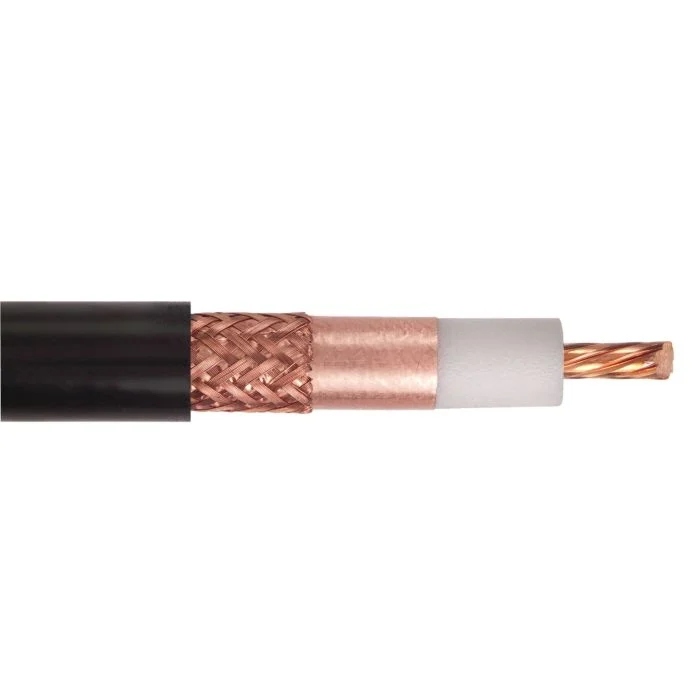
\includegraphics[scale = 0.5]{cavo coassiale vero.png}
\end{figure} 

\newpage 

\section{Campo EM in un cavo coax} 

\footnote{Slide del prof | PPT: Lezione 16 Mezzi trasmissivi 03 Maggio 23 | Pag 3-13}

\begin{figure}[h]
    \centering
    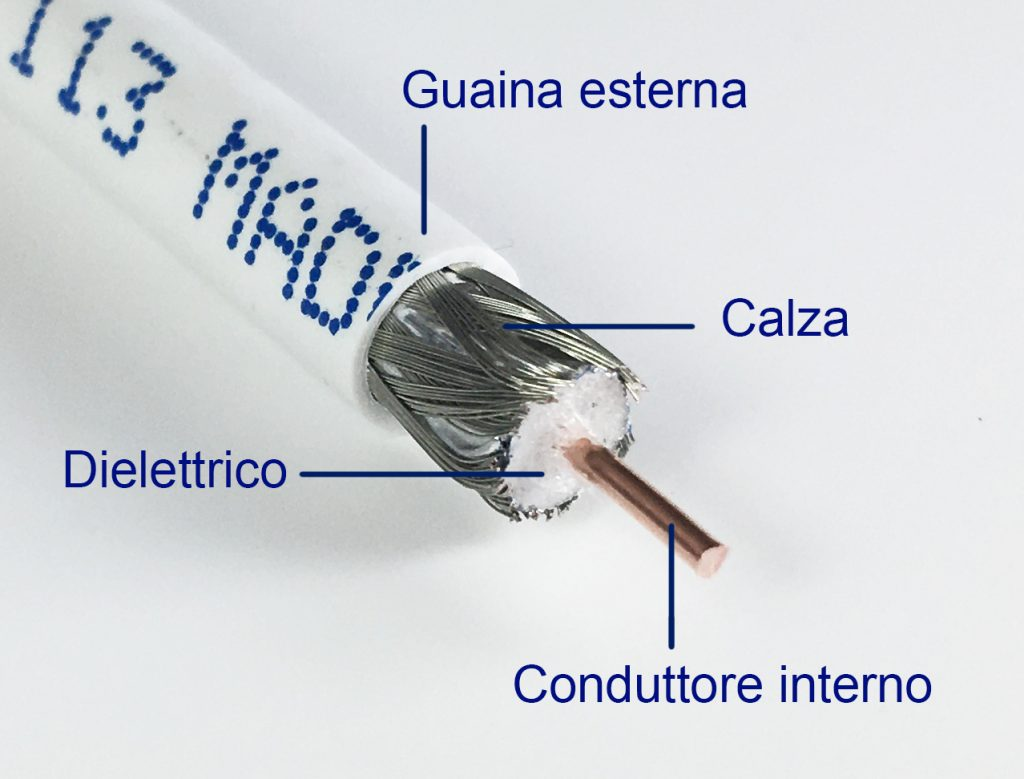
\includegraphics[scale = 0.5]{Cavo-spelato-nomi-delle-parti-copia-1024x779.jpg}
\end{figure} 

\footnote{\url{https://www.sistemi-integrati.net/cose-un-cavo-coassiale/}} 

Il cavo coassiale è un cavo cilindrico formato da (dall'interno all'esterno): 

\begin{itemize}
    \item condutore interno 
    \item dielettrico di separazione 
    \item calza conduttrice coassiale 
    \item guaina di protezione 
\end{itemize}

Essendo il cavo coassiale fisicamente di forma cilindrica, 
possiamo usare i fasori, in particolare le equazioni di Maxwell in forma 
fasoriale in assenza di sorgenti: 

{\Large \begin{equation}
    \begin{cases}
        \nabla \cdot \vec{E} = 0 \\ 
        \nabla \cdot \vec{H} = 0 \\
        \nabla \times \vec{E} = - \jmath \omega \mu \vec{H} \\ 
        \nabla \times \vec{H} = \jmath \omega \varepsilon \vec{E} 
    \end{cases}
\end{equation}}

Nella realtà non possiamo esprimere le equazioni delle onde in un cavo coassiale 
con le equazioni di Maxwell in assenza di sorgenti, ma adesso ci poniamo nel caso più 
semplice per svolgere i calcoli. \\ 

Sempre per quest'ultimo principio, consideriamo le onde polarizzate TEM, quindi: 

{\Large \begin{equation}
    \begin{cases}
        E_z = 0 \\ 
        H_z = 0
    \end{cases}
\end{equation}}

Considerando il cavo coassiale come cilindro, possiamo esprimere ogni punto del cavo 
in coordinate cilindriche: 

{\Large \begin{equation}
    (x, y, z) \Rightarrow (r, \phi, z )
\end{equation}}

\begin{tcolorbox}
    Dall'analisi matematica: 
    \begin{itemize}
        \item r indica il raggio 
        \item $\phi$ (si legge fi) indica i gradi  
    \end{itemize}
    Per approfondire\\
    \url{https://www.youmath.it/lezioni/analisi-due/varie/2282-coordinate-cilindriche.html} \\ 

    In questa sezione la notazione dei vettori indica quella di un fasore. 
\end{tcolorbox}

Vogliamo trovare una soluzione che non dipenda 
da $\phi$, quindi:
{\Large \begin{equation}
    \frac{\partial}{\partial \phi} = 0
\end{equation}} 

Essendo 
{
    \Large
     \begin{equation}
  E_z = 0      
     \end{equation}
}

$E_z$ è indipendete da $\phi$: 
questo principio prende il nome di simmetria azimutale. \\ 

Quindi possiamo scrivere che: 

{\Large \begin{equation}
    \nabla \cdot \vec{E} = 0 = \frac{1}{r} \frac{\partial}{\partial r} (r \vec{E_r} (r, z) )
\end{equation}}

Da questa equazione, notiamo che $\vec{E}$ dipende da r e da z. \\ 

Ritornando alla forma fisica del cavo coassiale, 
abbiamo due conduttori (il conduttore interno e la calza conduttrice coassiale) divisi 
da un dielettrico, proprio come un condensatore. \\ 

\begin{tcolorbox}
    Per approfondori sui condensatori \\
    \url{https://www.elettra2000.it/vdegliesposti/Dispense%20Propagazione/Richiami_Teoria_Dei_Circuiti.pdf}
\end{tcolorbox}
 
Applicando l'equazione costitutiva del condensatore al cavo coassiale, avremo che: 

{\Large \begin{equation}
    r \vec{E_r} (r, z) = Costante \cdot \vec{V} (z) 
    \Rightarrow \vec{E_r} (r, z) = \frac{Costante}{r} \vec{V} (z) 
\end{equation}}


\begin{figure}[h]
    \centering
    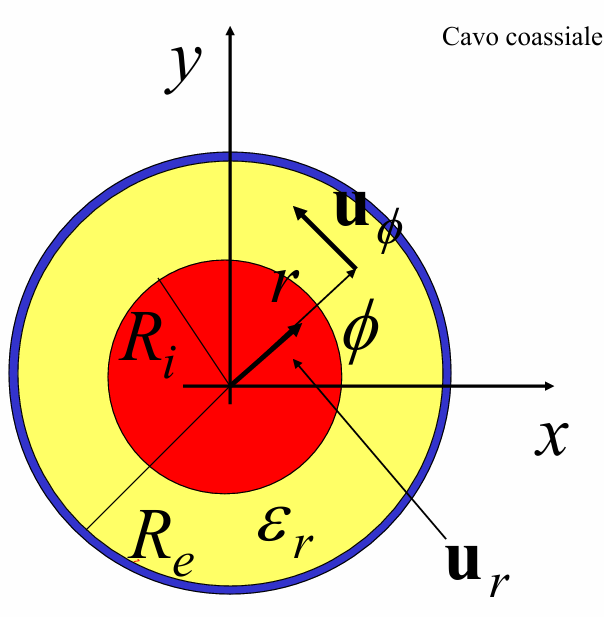
\includegraphics[scale = 0.5]{Cavo coax schematizzato.PNG}
\end{figure} 

\footnote{Slide del prof | PPT: Lezione 16 Mezzi trasmissivi 03 Maggio 23 | Pag 5} 

Proprio come il condensatore, facciamo un'intergrale di linea di un percorso chiuso tra le due armature, 
in questo caso tra i due conduttori: 

{\Large \begin{equation}
    \begin{split}
        \int_{R_i}^{R_e} \vec{E_r}(r, z) dr &= 
        \int_{R_i}^{R_e} \frac{Costante}{r} \vec{V} (z) dr \\
        & =  Costante \cdot \vec{V} (z) \int_{R_i}^{R_e} \frac{1}{r} dr \\ 
        & = Costante \cdot \vec{V} (z) \cdot \ln \left|r\right| \big|_{R_i} ^{R_e}   \\ 
        & =  Costante \cdot \vec{V} (z) \cdot \ln \left|R_e\right| - \\ 
        & Costante \cdot \vec{V} (z) \cdot \ln \left|R_i\right|  \\ 
        & = Costante \cdot \vec{V} (z) (\ln \left|R_e\right| - \ln \left|R_i\right|)  \\ 
        & = Costante \cdot \vec{V} (z) \ln \left|\frac{R_e}{R_i}\right|
    \end{split}
\end{equation}}

\begin{tcolorbox}
    $Costante \cdot \vec{V} (z)$ \\ 
    possiamo portarlo subito fuori dall'intergrale perchè 
    sono costanti rispetto a dr (r è l'incognita dell'integrale)   
\end{tcolorbox}

Alla fine avremo: 

{\Large \begin{equation}
    Costante \cdot \vec{V} (z) \ln \left|\frac{R_e}{R_i}\right| = \vec{V} (z)
\end{equation}}

Per essere vera questa ultima equazione: 

{\Large \begin{equation}
    Costante = \frac{1}{\ln \left|\frac{R_e}{R_i}\right|}
\end{equation}}

Sapendo ora il valore della costante possiamo esprimere $\vec{E_r}$ come: 

{\Large \begin{equation}
    \vec{E_r} (r, z) = \frac{Costante}{r} \vec{V} (z) 
    \Rightarrow \vec{E_r} (r, z) = \frac{1}{\ln \left|\frac{R_e}{R_i}\right|}  \frac{\vec{V} (z)}{r}
\end{equation}}

In "2.1 Equazioni dell'onda in forma fasoriale", abbiamo trovato che: 

{\Large \begin{equation}
    H_y = \frac{1}{- \jmath \omega \mu} \frac{\partial E_x}{\partial z}
\end{equation}}

In coordinate cilindriche, possiamo sostituire le rispettive coordinate, 
quindi $H_y$ diventa: 

{\Large \begin{equation}
    \vec{H_\phi} = \frac{1}{- \jmath \omega \mu} \frac{\partial E_r}{\partial z}
\end{equation}}

Sostitendo il valore di $\vec{E_r}$ trovato precedentemente, $\vec{H_\phi}$ diventa: 

{\Large \begin{equation}
    \vec{H_\phi} = \frac{1}{- \jmath \omega \mu} \frac{1}{r \ln \left|\frac{R_e}{R_i}\right| }\frac{\partial \vec{V} (z)}{\partial z}
\end{equation}}

Ritornando alle equazioni in forma fasoriale in coordinate cartesiane, sapevamo che: 

{\Large \begin{equation}
    \nabla \times \vec{H} = \jmath \omega \varepsilon \vec{E} 
    \Rightarrow \vec{E} = \frac{1}{\jmath \omega \varepsilon} \nabla \times \vec{H}
\end{equation}}

Sapendo il valore di $\vec{H}$, nell'asse x abbiamo che: 

{\Large \begin{equation}
    - \frac{\partial H_y}{\partial z} = \jmath \omega \varepsilon E_x 
    \Rightarrow E_x = - \frac{\partial H_y}{\partial z} \cdot \frac{1}{\jmath \omega \varepsilon}
\end{equation}}

Sostitendo a $x \Rightarrow r$ e $y \Rightarrow \phi$, avremo che: 

{\Large \begin{equation}
    \vec{E_r} (r, z) = - \frac{\partial H_\phi}{\partial z} \cdot \frac{1}{\jmath \omega \varepsilon}
\end{equation}}

Sapendo il valore di $H_\phi$, possiamo esprimere $\vec{E_r} (r, z)$ come: 

{\Large \begin{equation}
    \vec{E_r} (r, z) = - \frac{1}{r \ln \left|\frac{R_e}{R_i}\right|} \frac{1}{\kappa^{2}} \frac{\partial ^{2} \vec{V} (z)}{\partial  z^{2}}
\end{equation}}

Quindi è un'equazione che soddisfa l'equazione dell'onda: 

{\Large \begin{equation}
    \nabla ^{2} \vec{E} = -\kappa ^{2} \vec{E}
\end{equation}} 

dove: 

{\Large \begin{equation}
    \kappa ^{2} = \omega ^{2} \mu \varepsilon
\end{equation}} 

\newpage 

\section{Campo EM nel tempo}

\footnote{Slide del prof | PPT: Lezione 16 Mezzi trasmissivi 03 Maggio 23 | Pag 14 - 23}

Siccome le equazioni del campo EM soddisfano l'equazione dell'onda, 
possiamo esprimere la tensione come una sinusoide del tipo: 


{\Large  \begin{equation}
    \vec{E} (z) = V^{+} e^{-\jmath \kappa z} + V^{-} e^{+\jmath \kappa z}    
\end{equation}}


Ricordando che: 

{\Large \begin{equation}
    \vec{V} (z) = - \frac{1}{\kappa ^{2}} \frac{\partial^{2} \vec{V} (z)}{\partial z^{2}}
\end{equation}} 

e che: 

{\Large \begin{equation}
    \vec{E_r} (r, z) = \frac{1}{r \ln \left|\frac{R_e}{R_i}\right|} \vec{V}(z)
\end{equation}}

allora, possiamo convertire i fasori in quantità che variano nel tempo: 

{\Large \begin{equation}
    \begin{split}
        \Re{\vec{E_r} (r, z) e^{\jmath \kappa z}} 
        &= \frac{1}{r \ln \left|\frac{R_e}{R_i}\right|} \Re{\vec{V} (z) e^{\jmath \kappa z}} \\
        &= \frac{1}{r \ln \left|\frac{R_e}{R_i}\right|} V(z, t)
    \end{split}
\end{equation}}

dove: 

{\Large \begin{equation}
    \begin{split}
        V(z, t) 
        &=  \Re{\vec{V} (z) e^{\jmath \kappa z}} \\ 
        &= V^{+} \cos(\omega t - \kappa z) + V^{-} \cos(\omega t + \kappa z)     
    \end{split}
\end{equation}}

Come nel caso delle onde piane in forma fasoriale, possiamo descrivere V come somma 
di un'onda progressiva in direzione z e un'onda riflessa in direzione -z 

{\Large \begin{equation}
    \begin{split}
        V(z, t) &= f^{+} (t - \frac{z}{v}) + f^{-} (t + \frac{z}{v}) \\ 
        & = V^{+} \cos [\omega ( t - \frac{z}{v}) ] + V^{-} \cos [\omega ( t + \frac{z}{v}) ] 
    \end{split}
\end{equation}}

dove: 

{\Large \begin{equation}
    \begin{cases}
        v = \frac{\omega}{\kappa} 
        = \frac{\omega}{ \omega \sqrt{\mu \varepsilon}} 
        = \frac{1}{\sqrt{\mu \varepsilon}} 
        = c \\ 
        \lambda = \frac{2 \pi}{\kappa} 
        = \frac{2 \pi}{\omega} v 
        = \frac{v}{f}
    \end{cases}
\end{equation}}

Come le onde in forma fasoriale, $\vec{H_\phi}$ sarà: 

{\Large \begin{equation}
    \begin{split}
        \vec{H_\phi} &= \frac{1}{r \ln \left|\frac{R_e}{R_i}\right|} [V^{+} e^{-\jmath \kappa z} - V^{-} e^{\jmath \kappa z}] \\ 
        &= \sqrt{\frac{\varepsilon}{\mu}} \frac{1}{r \ln \left|\frac{R_e}{R_i}\right|} [V^{+} e^{-\jmath \kappa z} - V^{-} e^{\jmath \kappa z}]
    \end{split}
\end{equation}}

Come nelle onde piane, si può esprimere l'impedenza d'onda come: 

{\Large \begin{equation}
    \frac{\vec{E_r}^{+}}{\vec{H_\phi}^{+}} = 
    \sqrt{\frac{\mu_o}{\varepsilon}} = 
    \eta
\end{equation}}

Nel dominio del tempo $\vec{H_\phi}$ diventa: 

{\Large \begin{equation}
    \begin{split}
        \vec{H_\phi} (z, t) 
        &= \Re{\vec{H_\phi} e^{\jmath \omega t}} \\ 
        &= \sqrt{\frac{\varepsilon}{\mu}} \frac{1}{r \ln \left|\frac{R_e}{R_i}\right|} [V^{+} \cos(\omega t - \kappa z) - V^{-} \cos(\omega t + \kappa z)]
    \end{split}
\end{equation}} 

Sapendo ora il valore di $\vec{H_\phi}$,  
la corrente che fluisce nel conduttore interno è: 

{\Large \begin{equation}
    \begin{split}
        \vec{I} 
        &= \oint_{r = R_i} \vec{H_\phi} R_i d\phi \\
        &= \vec{H_\phi} \bigg|_{r = R_i} \cdot R_i \oint d\phi \\ 
        &= (\sqrt{\frac{\varepsilon}{\mu}} \frac{1}{r \ln \left|\frac{R_e}{R_i}\right|} [V^{+} \cos(\omega t - \kappa z) - V^{-} \cos(\omega t + \kappa z)]) \bigg|_{r = R_i} \cdot R_i \cdot 2\pi \\ 
        &= \sqrt{\frac{\varepsilon}{\mu}} \frac{1}{R_i \ln \left|\frac{R_e}{R_i}\right|} [V^{+} \cos(\omega t - \kappa z) - V^{-} \cos(\omega t + \kappa z)] \cdot R_i \cdot 2\pi \\ 
        &= 2\pi \sqrt{\frac{\varepsilon}{\mu}} \frac{1}{\ln \left|\frac{R_e}{R_i}\right|} [V^{+} \cos(\omega t - \kappa z) - V^{-} \cos(\omega t + \kappa z)] \\ 
        &=  I^{+} e^{- \jmath \kappa z} + I^{-} e^{+\jmath \kappa z}  
    \end{split}
\end{equation}} 

\begin{tcolorbox}
    Calcolare l'integrale di linea del percorso chiuso di un cerchio, in formula matematica \\ $\oint d\phi$ \\ 
    significa calcolare quanti radianti ci sono in un cerchio perchè l'incognita è 
    l'incognita $\phi$ e l'integrale è in $d\phi$. \\  \\ 
    Dalla geometria, i radianti di un qualsiasi cerchio, indipendentemente dal suo raggio, sono di $2 \pi$
\end{tcolorbox} 

\newpage 

\section{Costanti utili in un cavo coax} 

\footnote{Slide del prof | PPT: Lezione 16 Mezzi trasmissivi 03 Maggio 23 | Pag 24 - 29}

Una costante molto utile in un cavo coax  è la sua impedenza caratteristica: 

{\Large \begin{equation}
    \begin{split}
        Z_o 
        &= \frac{V^{+} e^{-\jmath \kappa z}}{I^{+} e^{-\jmath \kappa z}} = -\frac{V^{-} e^{+\jmath \kappa z}}{I^{-} e^{+\jmath \kappa z}} \\ 
        &= \frac{\sqrt{\frac{\mu}{\varepsilon}} \ln \left|\frac{R_e}{R_i}\right|}{2 \pi}
    \end{split}    
\end{equation}}

\begin{tcolorbox}
    Una piccola precisazione: \\ \\  
    l'impedenza caratteristica $Z_o$ dipende dalla tensione e dalla corrente 
    (da V e da I), quindi $Z_o$ dipende dal tipo di materiale utilizzato fisicamente nel cavo; \\ 
    a differenza dell'impendenza d'onda $\eta$ che dipende dal campo elettrico e dal campo magnetico 
    (da $\vec{E}$ e $\vec{H}$).      
\end{tcolorbox}


Quindi, possiamo esprimere la corrente in un punto z del cavo come: 
{\Large \begin{equation}
    \vec{I}(z)= \frac{1}{Z_o} [V^{+} e^{-\jmath \kappa z} - V^{-} e^{+\jmath \kappa z}]
\end{equation}} 

\begin{figure}[h]
    \centering
    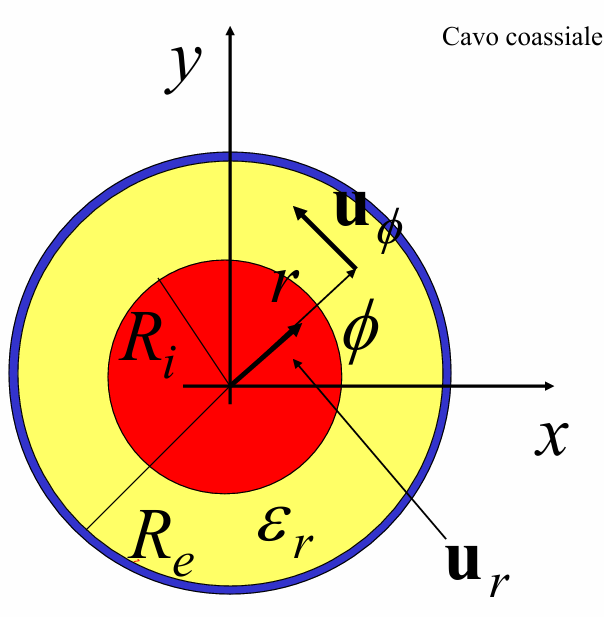
\includegraphics[scale = 0.5]{Cavo coax schematizzato.PNG}
\end{figure} 

\footnote{Slide del prof | PPT: Lezione 16 Mezzi trasmissivi 03 Maggio 23 | Pag 5} 

Visto che il cavo coassiale è formato da due conduttori, 
rispettivamente di raggio $R_i$ per il conduttore interno e di raggio $R_e$ per il conduttore esterno, 
divisi da un dielettrico, proprio come il condensatore, possiamo esprimere una carica per unità di lunghezza: 

{\Large \begin{equation}
    \begin{split}
        \hat{\rho_l} 
        &= \varepsilon \vec{E_r} (R_e, z) \hat{u_r} \cdot 2 \pi R_e \hat{u_r} \\ 
        &= \varepsilon \frac{1}{R_e \ln \left|\frac{R_e}{R_i}\right|} \vec{V} (z) \hat{u_r}  \cdot 2 \pi R_e \hat{u_r}
    \end{split}
\end{equation}}

dove l'unità di misura di $\hat{\rho_l}$ è: 

{\Large \begin{equation}
    [\hat{\rho_l} ] = \frac{C}{m}   
\end{equation}}

Proprio come il condensatore, possiamo esprimere la capacità per unità di lunghrzza come: 

{\Large \begin{equation}
    C = \frac{\hat{P_l}}{\hat{V} (z)} = \frac{2 \pi \varepsilon}{\ln \left|\frac{R_e}{R_i}\right|}
\end{equation}}

dove l'unità di misura di C è: 

{\Large \begin{equation}
    [C] = \frac{F}{m} 
\end{equation}} 

Essendo il cavo composto da due conduttori, possiamo esprimere il flusso di campo magnetico come: 

{\Large \begin{equation}
    \begin{split}
        \Phi_B 
        &= \mu_o \int_{R_i}^{R_e} \hat{H_\phi} dr \\  
        &= \mu_o \int_{R_i}^{R_e} \frac{\hat{I} (z)}{2 \pi} dr \\
        &= \mu_o \frac{\hat{I} (z)}{2 \pi} \ln \left|\frac{R_e}{R_i}\right| 
    \end{split}
\end{equation}} 

Quindi, possiamo esprimere l'induttanza per unità di lunghezza come: 

{\Large \begin{equation}
    L = \frac{\phi_B}{\hat{I}(z)} = \frac{\mu_o \ln \left|\frac{R_e}{R_i}\right|}{2 \pi}
\end{equation}}


Grazie ai valori di L e C, possiamo esprimere la velocità v, la costante di propagazione k e l'impedenza caratteristica $Z_o$: 

{\Large \begin{equation}
        Z_o = \sqrt{\frac{L}{C}} = \sqrt{\frac{\mu_o}{\varepsilon}} \frac{\ln \left|\frac{R_e}{R_i}\right| }{2 \pi} 
\end{equation}}

{\Large \begin{equation}
    v = \frac{1}{\sqrt{L C}} = \sqrt{\frac{2 \pi}{\mu_o \ln \left|\frac{R_e}{R_i}\right| } \cdot \frac{\ln \left|\frac{R_e}{R_i}\right|}{2 \pi \varepsilon}} = \frac{1}{\sqrt{\mu_o \varepsilon}}
\end{equation}} 

{\Large \begin{equation}
    \kappa = \omega \sqrt{L C} = \omega \sqrt{\mu_o \varepsilon}
\end{equation}}

\newpage 

\section{Teorema di Poynting in un cavo coax} 

\footnote{Slide del prof | PPT: Lezione 16 Mezzi trasmissivi 03 Maggio 23 | Pag 34-35}

Il teorema di Poynting è valido anche in un cavo coassiale. \\ 
Quindi, definiamo una superficie S ortogonale a $\hat{z}$: 

{\Large \begin{equation}
    \begin{split}
        \vec{S} 
        &= \vec{E} \times \vec{H}^{*} \\ 
        &= \frac{\hat{r} V(z)}{r \ln \left|\frac{R_e}{R_i}\right|}  \times \frac{\hat{\phi}}{2 \pi r} I^{*} (z) \\ 
        &= \frac{\hat{z}}{2 \pi r^{2} \cdot \ln \left|\frac{R_e}{R_i}\right|} V(z) I^{*} (z) 
    \end{split}
\end{equation}}

Dato S, possiamo calcolarci la potenza attiva trasportata da un'onda TEM in un cavo coax: 

{\Large \begin{equation}
    \begin{split}
        P &= \frac{1}{2} \Re{\int \int \vec{S} \cdot \hat{z} ds} \\ 
        &= \frac{1}{2} \Re{\int_{0}^{2 \pi} \int_{R_i}^{R_e} \vec{S} \cdot \hat{z} r dr d\phi} \\
        &= \frac{1}{2} \Re{V(z) I^{*} (z)} \\ 
        &= \frac{1}{2 Z_o} (\left|V^{+}\right| ^{2} - \left|V^{-}\right| ^{2})
    \end{split}
\end{equation}}

\newpage 

\section{Perdite nel dielettrico} 

\footnote{Slide del prof | PPT: Lezione 20 Perdite nel dieletrico 17 maggio 23 | Pag 3-4}

I due conduttori che costituiscono un cavo coax sono tenuti da un dielettrico con bassa permeattività 
(ad esempio il telflon). \\ 

\begin{tcolorbox}
Da \url{https://it.wikipedia.org/wiki/Permittivit%C3%A0_elettrica} \\
La permittività elettrica è una grandezza fisica che quantifica la tendenza del materiale a contrastare l'intensità del campo elettrico presente al suo interno. Descrive quindi il comportamento di un materiale in presenza di un campo elettrico. Viene anche comunemente chiamata costante dielettrica. \\ \\ 
La permittività elettrica è fortemente legata alla suscettività elettrica, ovvero alla predisposizione del materiale a polarizzarsi quando viene applicato un campo elettrico. La polarizzazione di atomi e molecole produce un campo elettrico aggiuntivo nel materiale, descritto attraverso il vettore induzione elettrica, e la permittività elettrica ne quantifica l'entità per unità di carica elettrica.    
\end{tcolorbox}

Quindi, il campo elettrico tra questi due conduttori è: 

{\Large \begin{equation}
    \vec{D} = \varepsilon_o \vec{E} + \vec{P_l}
\end{equation}}
 
dove $\vec{P_l}$ è la perdita del campo elettrico nel dielettrico. \\ \\ 

Se il mezzo è lineare: 

{\Large \begin{equation}
    \vec{P_l} = \varepsilon_o \chi_e \vec{E}
\end{equation}} 

\begin{tcolorbox}
    $\chi$ lettera greca che si legge chi
\end{tcolorbox}

dove $\chi_e$ tiene conto dell'energia EM dissipata sotto forma di calore. \\ \\ 

Permeattività complessa: 

{\Large \begin{equation}
    \begin{split}
        \varepsilon 
        &= \varepsilon_o (1 + \chi_e) \\ 
        &= \varepsilon_o \varepsilon_r (1 - \jmath \tan \delta)
    \end{split}
\end{equation}}

\begin{tcolorbox}
    $\delta$ lettera greca che si legge delta
\end{tcolorbox}

dove: 

$\delta$ è un parametro del dielettrico e non dipende dalla profondità di penetrazione. 

\begin{tcolorbox}
    Da \url{https://www.scienzaatscuola.it/fisica%205g/vivente3.html} \\ 
    La quantità $\delta$ è detta profondità di penetrazione e indica la distanza alla quale i campi si sono ridotti a circa il 37\% e la densità di potenza si è ridotta a meno del 14\% rispetto ai valori all'interfaccia. 
\end{tcolorbox}

Sapendo $\delta$, possiamo esprimere $\kappa$ come: 

{\Large \begin{equation}
    \begin{split}
        \kappa 
        &= \omega \sqrt{\mu_o \varepsilon} \\ 
        &\approx \omega \sqrt{\mu_o \varepsilon_o \varepsilon_r } (1 - \jmath \frac{\tan \delta}{2})    
    \end{split}
\end{equation}}

Inoltre, possiamo esprimere una costante di attenuazione del dielettrico $\alpha_d$ come: 

{\Large \begin{equation}
    \alpha_d \approx \kappa \frac{\tan \delta}{2}
\end{equation}}

Oltre al dielettrico, il cavo coax presente due conduttori, quindi possiamo 
esprimere una costante di attenuazione del conduttore $\alpha_c$ come: 

{\Large \begin{equation}
    \begin{split}
        \alpha_c 
        &= \frac{P_l (z)}{2P(z)} \\ 
        &\approx \frac{\frac{R_s}{4 \pi} [\frac{1}{R_i} + \frac{1}{R_e}]}{Z_o} \\ 
        &= \frac{\frac{R_s}{4 \pi R_i} [1 + \frac{R_i}{R_e}]}{\frac{\eta}{2 \pi} \ln \left|\frac{R_e}{R_i}\right|}
    \end{split}
\end{equation}} 

dove: 

{\Large \begin{equation}
    \begin{cases}
        R_s = \frac{1}{\sigma \delta} \\ 
        \delta = \frac{1}{\sqrt{\pi f \mu_o \sigma}}
    \end{cases}
\end{equation}}

\begin{tcolorbox}
    $\delta$ lettera greca si legge delta
\end{tcolorbox}

Spesso, è preferibile esprimere le perdite totali in un cavo coax in dB: 

{\Large \begin{equation}
    \alpha_{dB} = -20 \log e^{- (\alpha_c + \alpha_d)}
\end{equation}} 

\newpage 

\section{Perdite dipendenti dalla temperatura nel dielettrico}

\footnote{Slide del prof | PPT: Lezione 20 Perdite nel dieletrico 17 maggio 23 | Pag 15}

La temperatura influisce sul coefficiente elettrico di attenuazione $\alpha(T)$: 

{\Large \begin{equation}
    \alpha (T) = \alpha_{293 K} \cdot \sqrt{1 + \sigma_P (\frac{T}{K} - 293)}
\end{equation}}


dove: 
\begin{itemize}
    \item $\alpha_P$ è il coefficiente di resistività (è un parametro empirico riguardo al materiale del conduttore) 
    \item $\alpha_{293 K}$  è la resistività a 293 Kelvin 
\end{itemize}

Se il cavo coax è corto circuitato: 

{\Large \begin{equation}
    V^{+} = -V^{-}
\end{equation}} 

Quindi: 

{\Large \begin{equation}
    V_{max} = 2 \left|V^{+}\right|
\end{equation}}

\newpage 

\chapter{Guide d'onda} 

\begin{figure}[h]
    \centering
    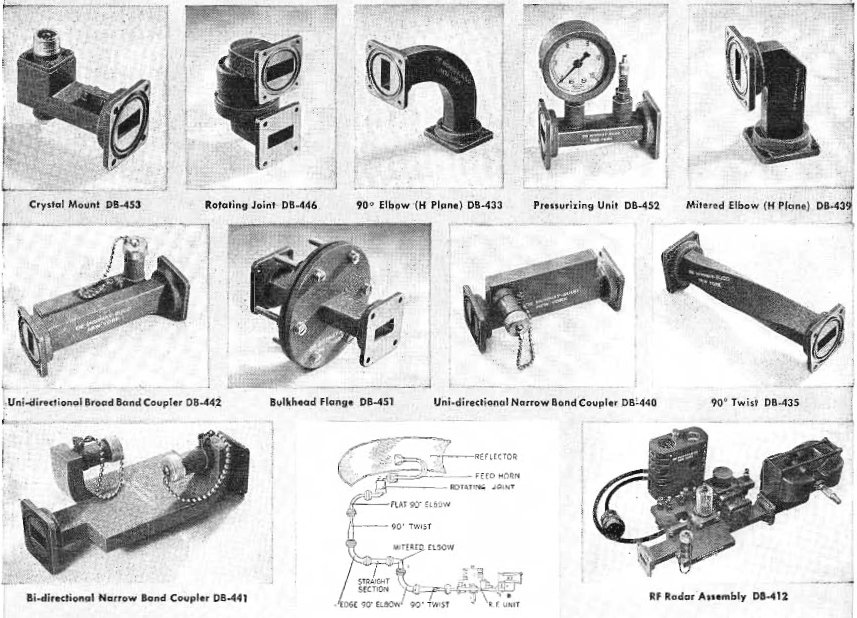
\includegraphics[scale = 0.5]{Waveguide_collection.jpg}
\end{figure} 

\newpage 

\section{Cosa sono le guide d'onda} 

\footnote{FWC - pag 395 \\ 8.1 Introduction}

La guida d'onda è una struttura, o parte di una struttura, che permette 
ad un'onda di propagarsi in una precisa direzione. \\ 

Se la guida d'onda cambia direzione, l'onda è costretta a seguirla. \\ 

I componenti trasversali dell'onda si propagheranno lungo la direzione di propagazione. \\ 

Generalmente, nelle analisi delle guide d'onda, siamo interessati alla distribuzione dei campi EM; 
ma, la cosa più importante è la dipendenza della costante di propagazione rispetto alla frequenza. \\ 

Dalla costante di propagazione è possibile calcolare la velocità dell'onda, 
la variazione di fase e l'attenuazione lungo la guida d'onda. \\ 

\newpage 

\section{Equazioni delle guide d'onda per sistemi uniformi} 
\footnote{FWC - pag 396 \\ 8.2 Basic equations and wave types for uniform systems}

Nelle guide d'onda considereremo onde del tipo: 

{\Large 
    \begin{equation}
        e^{\jmath \omega t - \gamma z}
    \end{equation}
}

quindi onde a tempo armonico $\jmath \omega t$ e che variano con la distanza $ - \gamma z$. \\ \\ 


\begin{tcolorbox}
    $\gamma$ dall'alfabeto greco si legge gamma 
\end{tcolorbox}


La costante di propagazione $\gamma$ sarà importante per le proprietà dell'onda, 
come ad esempio di quanto si attenua l'onda, la fase e la velocità di gruppo. \\ \\ 

Assumiamo nessuna densità di carica in ingresso e considereremo i conduttori della guida d'onda soddisfino l'equazione: 

{
    \Large
    \begin{equation}
        \kappa^{2} = \omega^{2} \mu \varepsilon
    \end{equation}
} 

Le equazioni dell'onda, che si riducono alle equazioni di Helmholtz per i campi fasoriali, saranno: 

{
    \Large 
    \begin{equation}
        \begin{cases}
            \nabla ^{2} \vec{E} = - \kappa ^{2}  \vec{E} \\ 
            \nabla ^{2} \vec{H} = - \kappa ^{2}  \vec{H} \\    
        \end{cases}
    \end{equation}
}

Nelle coordinate cartesiane, $\nabla ^{2}$, chiamato anche operatore di Laplace, può essere suddiviso in due parti: 

{
    \Large 
    \begin{equation}
        \begin{split}
            \nabla ^{2} \vec{E} 
            &= \frac{\partial ^{2} \vec{E}}{\partial x ^{2}} + \frac{\partial ^{2} \vec{E}}{\partial y ^{2}} + \frac{\partial ^{2} \vec{E}}{\partial z ^{2}}
            \\
            &= \nabla_t ^{2} \vec{E} + \frac{\partial ^{2} \vec{E}}{\partial z^{2}}  
        \end{split}
    \end{equation}
} 

dove, $\nabla_t ^{2}$ lo definiamo come operatore di Laplace trasversale. \newline 

Assumendo la funzione di propagazione lungo l'asse x $e^{-\gamma z}$, possiamo scrivere: 

{
    \Large
    \begin{equation} 
        \frac{\partial ^{2} \vec{E}}{\partial z^{2}} = \gamma ^{2} \vec{E}
    \end{equation}
}

Uguagliando i due modi di esprimere $\nabla ^{2} \vec{E}$ e sostituendo il 
valore di $ \frac{\partial ^{2} \vec{E}}{\partial z^{2}}$, possiamo scrivere la seguente equazione: 

{
    \Large 
    \begin{equation}
        \begin{cases}
            \nabla ^{2} \vec{E} = - \kappa ^{2}  \vec{E} \\
            \nabla ^{2} \vec{E} = \nabla_t ^{2} \vec{E} + \frac{\partial ^{2} \vec{E}}{\partial z^{2}}
        \end{cases} 
        \Rightarrow
        - \kappa ^{2}  \vec{E} = \nabla_t ^{2} \vec{E} + \gamma ^{2} \vec{E}
    \end{equation}
}

Oppure, svolgendo diversi passi algebrici: 

{
    \Large
    \begin{equation}
        \begin{split}
            \nabla_t ^{2} \vec{E} 
            &= - \kappa ^{2}  \vec{E} - \gamma ^{2}  \vec{E} \\ 
            &= -(\kappa ^{2} + \gamma ^{2}) \vec{E} 
        \end{split}
    \end{equation}
}

I passaggi algebrici svolti per $\nabla_t ^{2} \vec{E}$ possono essere svolti 
anche per $\nabla_t ^{2} \vec{H}$: 

{
    \Large
    \begin{equation}
        \nabla_t ^{2} \vec{H} = -(\kappa ^{2} + \gamma ^{2}) \vec{H}
    \end{equation}
}

$\nabla_t ^{2} \vec{E}$ e $\nabla_t ^{2} \vec{H}$ sono equazioni differenziali che devono essere soddisfatte 
nelle regione del dielettrico della linea di trasmissione o della guida d'onda. \\ 


La procedura standard è quella di trovare i componenti di $\vec{E}$ e $\vec{H}$ lungo 
l'asse z che soddisfano $\nabla_t ^{2} \vec{E}$ e $\nabla_t ^{2} \vec{H}$, quindi le condizioni al contorno, oppure 
esplicitato in una maniera differente, troviamo $E_z$ e $H_z$ in modo tale che siano le variabili indipendenti del sistema. \\ 

Consideriamo le equazioni di $e^{\jmath \omega t - \gamma z}$ 
in forma fasoriale divise nei loro componenti. \\ 

Dalle leggi di Maxwell avremo: 

{
    \Large 
    \begin{equation}
            \nabla \times \vec{E} 
            = \operatorname{rot}
            \begin{vmatrix}
                \hat{x} & \hat{y} &\hat{z} \\ \\ 
                \frac{\partial}{\partial x} & \frac{\partial}{\partial y} & -\gamma \\ \\ 
                E_x & E_y & E_z
            \end{vmatrix}  
    \end{equation}
}

Svolgendo diversi passi algebrici: 

{
    \Large 
    \begin{equation}
        \nabla \times \vec{E} 
            = 
            \hat{x} 
            \begin{vmatrix}
            \frac{\partial}{\partial y} & -\gamma \\  \\ 
            E_y & E_z 
            \end{vmatrix}
            -\hat{y} 
            \begin{vmatrix}
            \frac{\partial}{\partial x} & -\gamma \\  \\ 
            E_x & E_z 
            \end{vmatrix}
            +\hat{z} 
            \begin{vmatrix}
            \frac{\partial}{\partial x} & \frac{\partial}{\partial y} \\  \\ 
            E_x & E_y 
            \end{vmatrix}
    \end{equation}
}

{
    \Large 
    \begin{equation}
            \nabla \times \vec{E}
            = 
            \hat{x} 
            [
                \frac{\partial E_z}{\partial y} 
                +\gamma E_y
            ]    
            -\hat{y} 
            [
                \frac{\partial E_z}{\partial x} 
                +\gamma E_x
            ]    
            +\hat{z} 
            [
                \frac{\partial E_y}{\partial x} 
                + \frac{\partial E_x}{\partial y}
            ] 
    \end{equation}
}

{
    \Large 
    \begin{equation}
            \nabla \times \vec{E}
            =        
\hat{x} 
[
    \frac{\partial E_z}{\partial y} 
    +\gamma E_y
]    
+\hat{y} 
[
    -\frac{\partial E_z}{\partial x} 
    -\gamma E_x
]    
+\hat{z} 
[
    \frac{\partial E_y}{\partial x} 
    + \frac{\partial E_x}{\partial y}
] 
    \end{equation}
}       


Dalle equazioni di Maxwell in forma fasoriale: 

{
    \Large 
    \begin{equation}
        \nabla \times \vec{E} = -\jmath \omega \mu \vec{H}
    \end{equation}
}

Divendendo questa equazione nei vari assi cartesiani: \\ 

\textbf{Asse X} 

{
    \Large 
    \begin{equation}
        \frac{\partial E_z}{\partial y} + \gamma E_y 
        = 
        -\jmath \omega \mu H_x
    \end{equation}
}


\textbf{Asse Y} 

{
    \Large 
    \begin{equation}
        - \gamma E_x - \frac{\partial E_z}{\partial x}  
        = 
        -\jmath \omega \mu H_y
    \end{equation}
}



\textbf{Asse Z} 

{
    \Large 
    \begin{equation}
        \frac{\partial E_y}{\partial x} - \frac{\partial E_x}{\partial y} 
        = 
        -\jmath \omega \mu H_z
    \end{equation}
}

Sostituendo $\vec{H}$ ad $\vec{E}$, possiamo trovare le equazioni 
di Maxwell in forma fasoriale di: 

Dalle equazioni di Maxwell in forma fasoriale: 

{
    \Large 
    \begin{equation}
        \nabla \times \vec{H} = \jmath \omega \varepsilon \vec{E}
    \end{equation}
}


\textbf{Asse X} 

{
    \Large 
    \begin{equation}
        \frac{\partial H_z}{\partial y} + \gamma H_y 
        = 
        \jmath \omega \varepsilon E_x
    \end{equation}
}


\textbf{Asse Y} 

{
    \Large 
    \begin{equation}
        - \gamma H_x - \frac{\partial H_z}{\partial x}  
        = 
        \jmath \omega \varepsilon E_y
    \end{equation}
}



\textbf{Asse Z} 

{
    \Large 
    \begin{equation}
        \frac{\partial H_y}{\partial x} - \frac{\partial H_x}{\partial y} 
        = 
        \jmath \omega \varepsilon E_z
    \end{equation}
}

Ora è possibile trovare $E_x$, $E_y$, $H_x$, $H_y$ 
in funzione di $E_z$ e $H_z$. \\ 

I passaggi algebrici sono omessi, però basta sostituire i valori. \\ 

Alla fine troveremo i i valori di: 

{
    \Large 
    \begin{equation}
        \begin{cases}
            E_x = - \frac{1}{\gamma ^{2} + \kappa ^{2}} (\gamma \frac{\partial E_z}{\partial x} + \jmath \omega \mu \frac{\partial H_z}{\partial y}) \\ \\ 
            E_y =  \frac{1}{\gamma ^{2} + \kappa ^{2}} (- \gamma \frac{\partial E_z}{\partial y} + \jmath \omega \mu \frac{\partial H_z}{\partial x}) \\ \\ 
            H_x =  \frac{1}{\gamma ^{2} + \kappa ^{2}} (- \gamma \frac{\partial H_z}{\partial x} + \jmath \omega \varepsilon \frac{\partial E_z}{\partial y}) \\ \\ 
            H_y =  -\frac{1}{\gamma ^{2} + \kappa ^{2}} ( \gamma \frac{\partial H_z}{\partial y} + \jmath \omega \varepsilon \frac{\partial E_z}{\partial x}) 
        \end{cases}
    \end{equation}
}

È conveniente scrivere: 

{
    \Large
    \begin{equation}
        \begin{cases}
            \gamma = \jmath \beta \\ 
            \kappa_c ^{2} = \gamma^{2} + \kappa^{2} = \kappa^{2} - \beta^{2} 
        \end{cases}
    \end{equation}
}



Le equazioni precedentemente scritte, diventeranno: 

{
    \Large 
    \begin{equation}
        \begin{cases}
            E_x = - \frac{\jmath}{\kappa_c ^{2}} (\beta \frac{\partial E_z}{\partial x} + \omega \mu \frac{\partial H_z}{\partial y}) \\ \\ 
            E_y =  \frac{\jmath}{\kappa_c ^{2}} (- \beta \frac{\partial E_z}{\partial y} + \omega \mu \frac{\partial H_z}{\partial x}) \\ \\ 
            H_x =  \frac{\jmath}{\kappa_c ^{2}} (- \beta \frac{\partial H_z}{\partial x} + \omega \varepsilon \frac{\partial E_z}{\partial y}) \\ \\ 
            H_y =  -\frac{\jmath}{\kappa_c ^{2}} ( \beta \frac{\partial H_z}{\partial y} + \omega \varepsilon \frac{\partial E_z}{\partial x}) 
        \end{cases}
    \end{equation}
}

Inoltre possiamo scrivere: 

{
    \Large 
    \begin{equation}
        \begin{cases}
            \nabla_t ^{2} E_z = - \kappa_c ^{2} E_z \\ \\
            \nabla_t ^{2} H_z = - \kappa_c ^{2} H_z     
        \end{cases}
    \end{equation} 
}

\newpage
\chapter{Guide d'onda rettangolari} 

\begin{figure}[h]
    \centering
    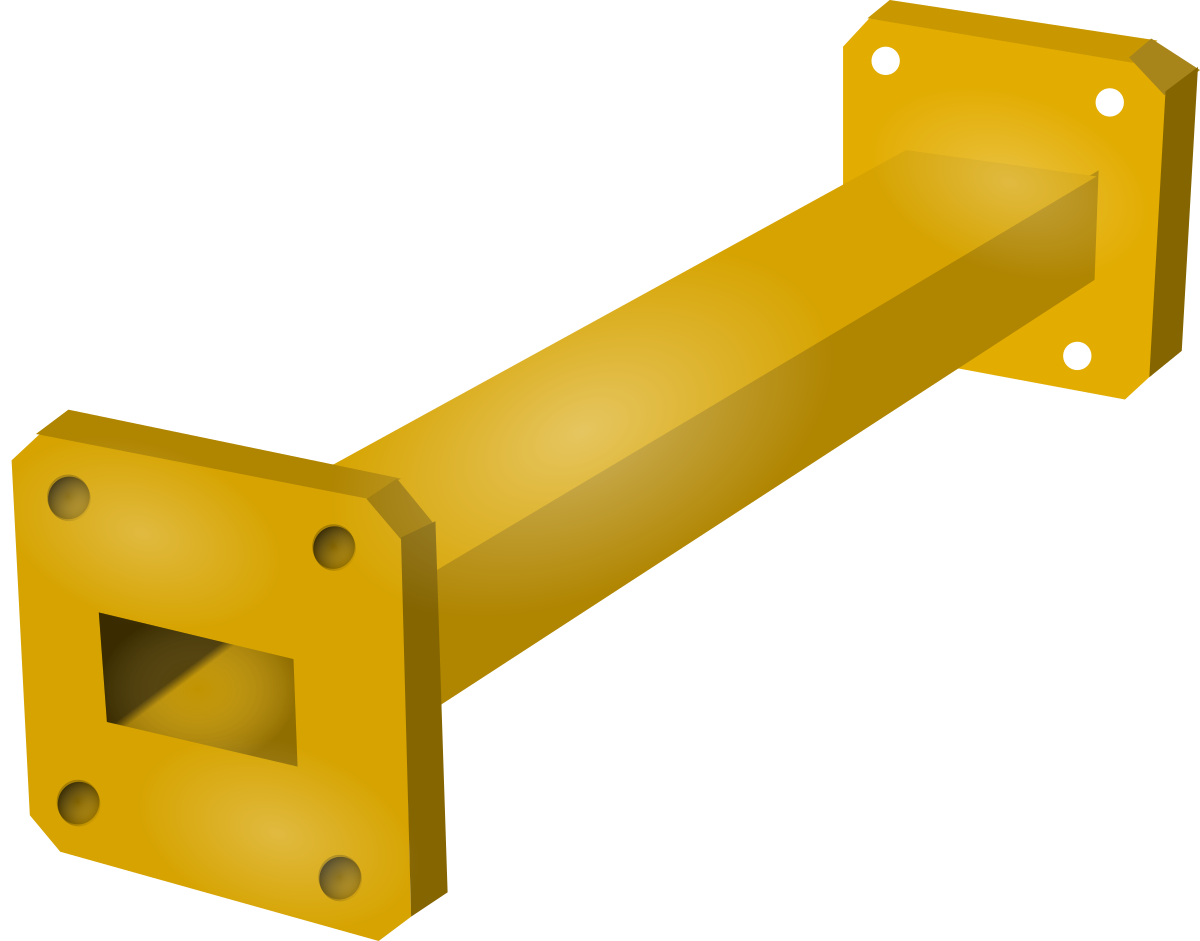
\includegraphics[scale = 0.35]{Waveguide17-with-UBR120-flanges-svg.svg.png}
\end{figure} 

\newpage 

\section{Cosa sono le guide d'onda rettangolari} 

\footnote{FWC - pag 417 \\ 8.7 Rectangular waveguides}

\begin{figure}[h]
    \centering
    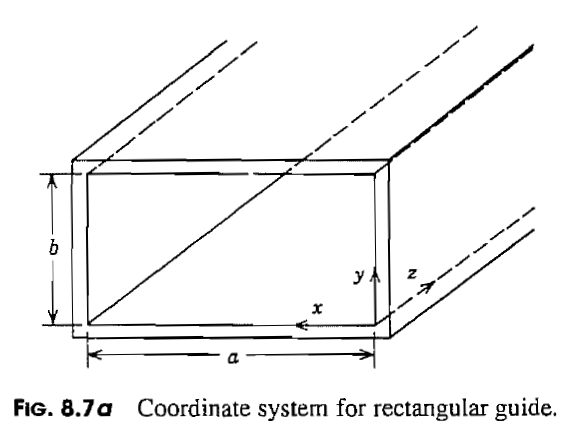
\includegraphics{Coordinate system for rectangular guide.PNG}
\end{figure} 

Le onde rettangolari sono un tipo d'onda in cui la sezione è formata da una regione dielettrica di larghezza 
a e di altezza b che si estende per una lunghezza infinita lungo la direzione z, 
regione dielettrica rivestita da quattro conduttori. \\ 

Non ci possono essere onde TEM perchè la componente lungo z non varia (considerando che nella guida d'onda possono 
esistere onde del tipo $e^{-\jmath \omega t - \gamma z}$ e che quindi variano di $\gamma$ lungo l'asse z). \\ 

Onde TM e TE possono esistere in una guida d'onda rettangolare. 

\newpage 

\section{Onde TM nelle guide d'onda rettangolari} 

\footnote{FWC - pag 418 \\ 8.7 Rectangular waveguides - TM Waves} 

Le onde TM, lungo la componente dell'asse z: 

{
    \Large 
    \begin{equation}
        \begin{cases}
            H_z = 0 \\ 
            E_z \neq 0
        \end{cases}
    \end{equation}
}

Dalle equazioni di Maxwell per le guide d'onda, abbiamo trovato che: 

{
    \Large 
    \begin{equation}
        \nabla_t ^{2} E_z 
        = \frac{\partial ^{2} E_z}{\partial x^{2}} + \frac{\partial ^{2} E_z}{\partial y^{2}}
        = - \kappa_c ^{2} E_z
    \end{equation}
}

dove: 

{
    \Large 
    \begin{equation}
        \kappa_c ^{2} = \kappa_x ^{2} + \kappa_y ^{2}
    \end{equation}
}

Quindi: 

{
    \Large 
    \begin{equation}
        \frac{\partial ^{2} E_z}{\partial x^{2}} + \frac{\partial ^{2} E_z}{\partial y^{2}}
        = - \kappa_c ^{2} E_z
        \Rightarrow 
        \frac{\partial ^{2} E_z}{\partial x^{2}} + \frac{\partial ^{2} E_z}{\partial y^{2}}
        =  - \kappa_x ^{2} - \kappa_y ^{2} E_z
    \end{equation}
}

Utilizzando la separazione delle variabili (x,y) possiamo portare questa 
equazione in un sistema per ogni variabile, cioè: 

{
    \Large
    \begin{equation}
        \begin{cases}
            \frac{\partial ^{2} E_z}{\partial x^{2}} 
            = - \kappa_x ^{2} E_z \\ \\
            \frac{\partial ^{2} E_z}{\partial y^{2}} 
            = - \kappa_y ^{2} E_z  
        \end{cases}
    \end{equation}
}


Il cui risultato è rispettivamente \\ 
per l'asse x: 

{
    \Large 
    \begin{equation}
        A^{'} \sin(\kappa_x x) + B^{'} \cos(\kappa_x x) 
    \end{equation}
}

per l'asse y: 

{
    \Large 
    \begin{equation}
        C^{'} \sin(\kappa_y y) + D^{'} \cos(\kappa_y y) 
    \end{equation}
}

dove $A^{'}$, $B^{'}$, $C^{'}$, $D^{'}$ sono coefficienti reali. \\ 

La separazione delle variabili ci impone di moltiplicare i risultati 
per l'asse x e l'asse y, quindi $E_z$ diventa: 

{
    \Large 
    \begin{equation}
        E_z 
        = 
        (A^{'} \sin(\kappa_x x) + B^{'} \cos(\kappa_x x))  (C^{'} \sin(\kappa_y y) + D^{'} \cos(\kappa_y y))
    \end{equation}
}

Siccome consideriamo le pareti della guida d'onda come perfetti conduttori, 
$E_z = 0$ in: 

{
    \Large 
    \begin{equation}
        \begin{cases}
            x = 0 \\ 
            y= 0
        \end{cases}
    \end{equation}
} 

Allora: 

{
    \Large 
    \begin{equation}
        \begin{cases}
            B^{'}= 0 \\ 
            D^{'}= 0
        \end{cases}
    \end{equation}
} 

Ponendo: 

{
    \Large 
    \begin{equation}
            A^{'}C^{'} = A 
    \end{equation}
} 

e considerando le semplificazioni svolti, $E_z$ diventerà: 

{
    \Large 
    \begin{equation}
        E_z = A \sin(\kappa_x x) \sin(k_y y)
    \end{equation}
}

Per $A \neq 0$, $E_z = 0$ non solo in (0, 0), ma anche in: 

{
    \Large 
    \begin{equation}
        \begin{cases}
            x = a \\ 
            y= b
        \end{cases}
    \end{equation}
}

Essendo il $\sin$ una funzione sinusoidale, possiamo scrivere che
$E_z = 0$ non solo per in (a, b) ma anche in: 

{
    \Large
    \begin{equation}
        \begin{cases}
            \sin(\kappa_x x) = 0 
            \Rightarrow 
            \kappa a = m \pi \\ 
            \sin(\kappa_y y) = 0 
            \Rightarrow 
            \kappa b = n \pi 
        \end{cases}
    \end{equation}
}

dove m e n è un numero intero maggiore di 0. \\ 

Quindi per un'onda $TM_{n m}$, la frequanza di cut-off, cioè 
la frequenza per cui $E_z = 0$ è: 


{
    \Large 
    \begin{equation}
        \begin{split}
            \omega_{c_{m,n}} 
            &= 
            \frac{\kappa_{c_{m,n}}}{\sqrt{\mu \varepsilon}} \\
            &= 
            \frac{1}{\sqrt{\mu \varepsilon}} \sqrt{[(\frac{n \pi}{a}) ^{2} + (\frac{m \pi}{b}) ^{2}]}    
        \end{split}
    \end{equation}
}

Siccome sappiamo che: 

{
    \Large 
    \begin{equation}
        \kappa_c ^{2} = \kappa^{2} - \beta^{2}
    \end{equation}
}

è possibile trovare la costante di fase per le frequenze 

{
    \Large 
    \begin{equation}
        \begin{cases}
            \alpha 
            = 
            \kappa_{c_{m,n}} \sqrt{1 - (\frac{\omega}{\omega_{c_{m,n}}})} 
            \text{  per } 
            \omega < \omega_{c_{m,n}}
            \\ \\
            \beta
            = 
            \kappa \sqrt{1 - (\frac{\omega_{c_{m,n}}}{\omega})} 
            \text{  per } 
            \omega > \omega_{c_{m,n}}
        \end{cases}
    \end{equation}
}

La velocità di fase di gruppo sono rispettivamente: 

{
    \Large
    \begin{equation}
        \begin{cases}
            v_p 
            = 
            \frac{\omega}{\beta} 
            = 
            \frac{v}{\sqrt{1 - (\frac{\omega_{c_{m,n}}}{\omega})}}
            \\ \\
            v_g 
            = 
            \frac{ d \omega}{ d \beta} 
            = 
            v\sqrt{1 - (\frac{\omega_{c_{m,n}}}{\omega})}
        \end{cases}
    \end{equation}
}

\begin{tcolorbox}
    In fisica la velocità di fase è la velocità con cui si propaga la fase di un'onda, sia essa elettromagnetica o meccanica. La velocità di fase può essere visualizzata come la velocità di propagazione di una cresta dell'onda ma non coincide necessariamente con la velocità di propagazione di un segnale (che è più propriamente descritta dalla velocità di gruppo) e quindi può essere più alta della velocità della luce senza violare la relatività ristretta. \\
    \url{https://it.wikipedia.org/wiki/Velocit%C3%A0_di_fase} \\ \\
    La velocità di gruppo di un'onda è la velocità con cui si propagano nello spazio le variazioni nella forma dell'ampiezza dell'onda. \\
    La velocità di gruppo è spesso considerata la velocità a cui l'energia o l'informazione sono trasportate dall'onda. In molti casi questa è una visione accurata, e la velocità di gruppo può essere pensata come la velocità di segnale della forma d'onda. \\
    \url{https://it.wikipedia.org/wiki/Velocit%C3%A0_di_gruppo}
\end{tcolorbox}

\newpage 

\section{Onde TE nelle guide d'onda rettangolari} 

\footnote{FWC - pag 419 \\ 8.7 Rectangular waveguides - TE Waves}

Il procedimento sarà simile al caso precedente delle onde TM, ma cambieranno alcune cose. \\ 

Prima di tutto, nelle onde TE abbiamo che: 

{
    \Large 
    \begin{equation}
        \begin{cases}
            H_z \neq 0 \\ 
            E_z = 0
        \end{cases}
    \end{equation}
}

Inoltre: 
{
    \Large 
    \begin{equation}
        \nabla_t ^{2} H_z 
        = \frac{\partial ^{2} H_z}{\partial x^{2}} + \frac{\partial ^{2} H_z}{\partial y^{2}}
        = - \kappa_c ^{2} H_z
    \end{equation}
}

Facendo lo stesso procedimento della separazione delle variabili del caso TE, abbiamo che: 

{
    \Large 
    \begin{equation}
        H_z 
        = 
        (A^{'} \sin(\kappa_x x) + B^{'} \cos(\kappa_x x)) (C^{'} \sin(\kappa_y y) + D^{'} \cos(\kappa_y y))
    \end{equation}
}

I vari componenti dell'onda saranno: 

{
    \Large
    \begin{equation}
        \begin{split}
            E_x 
            &= 
            -\frac{\jmath \omega \mu}{\kappa_c ^{2}} \frac{\partial H_z}{\partial y}
            \\ \\ \\
            &= 
            - \frac{\jmath \omega \mu \kappa_y}{\kappa_c ^{2}} (A^{'} \sin(\kappa_x x) + B^{'} \cos(\kappa_x x)) (C^{'} \cos(\kappa_y y) - D^{'} \sin(\kappa_y y))
        \end{split}
    \end{equation}
}

{
    \Large
    \begin{equation}
        \begin{split}
            E_y 
            &= 
            \frac{\jmath \omega \mu}{\kappa_c ^{2}} \frac{\partial H_z}{\partial x}
            \\ \\ \\
            &= 
            \frac{\jmath \omega \mu \kappa_x}{\kappa_c ^{2}} (A^{'} \cos(\kappa_x x) - B^{'} \sin(\kappa_x x)) (C^{'} \sin(\kappa_y y) + D^{'} \cos(\kappa_y y))
        \end{split}
    \end{equation}
}

In questo caso, però: 

{
    \Large
    \begin{equation}
        \begin{cases}
            E_x = 0 \text{  per } (x, 0) \Rightarrow C^{'} = 0 \\ 
            E_x = 0 \text{  per } (0, y) \Rightarrow A^{'} = 0 \\ 
        \end{cases}
    \end{equation}
}

Ponendo: 

{
    \Large 
    \begin{equation}
        B = B^{'}D^{'}
    \end{equation}
}

$H_z$ diventa: 

{
    \Large 
    \begin{equation}
        H_z = B \cos(\kappa_x x)\cos(\kappa_y y)
    \end{equation}
}

Per $E_x = 0$ in $y=b$ ,quindi: 

{
    \Large
    \begin{equation}
        \kappa_y b = n \pi
    \end{equation}
}

Per $E_y = 0$ in $x=a$ ,quindi: 

{
    \Large
    \begin{equation}
        \kappa_x a = m \pi
    \end{equation}
}

A differenza delle onde TM, basta solo che sia soddisfatta 
solo una delle due condizioni elencate precedentemente per avere continuità 
dell'onda. \\ 

$\omega_{c_{m,n}}$, $\alpha$, $\beta$, $v_p$ e $v_g$ sono le stesse della $TM_{n, m}$ 

\newpage 
 
\chapter{Modi di guida d'onda rettangolare} 

\begin{figure}[h]
    \centering
    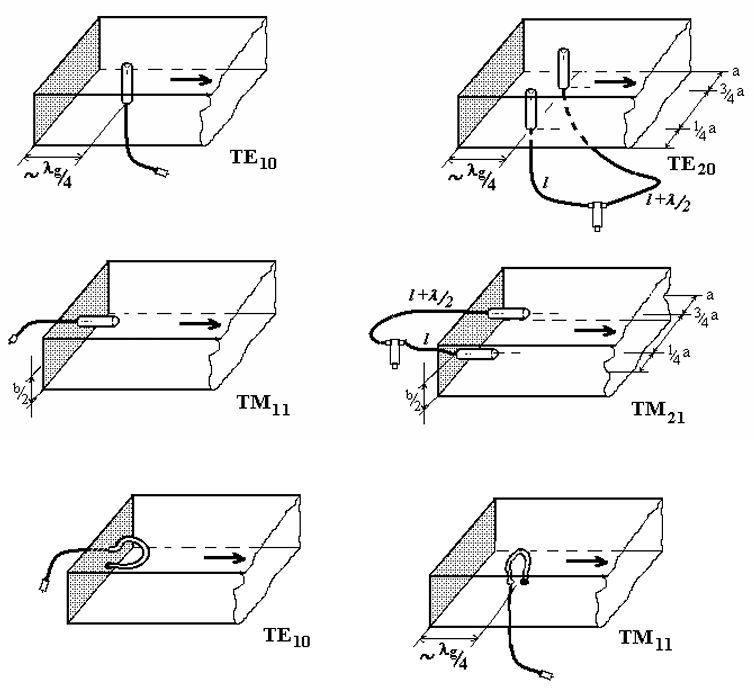
\includegraphics[scale = 0.9]{Modi di guida rettangolare.PNG}
\end{figure}  

\newpage 

\section{Modo fondamentale: $TE_{10}$}

\footnote{Slide del prof | PPT: Lezione 21 - 22 Guide rettangolari 22-24 maggio 2023 | Pag 13-20 \\ 
FWC - pag 422 \\
FWC - 8.8 The $TE_{10}$ wave in a rectangular guide - pag 423 \\
Ricevimento con prof}

\begin{tcolorbox}
    $TE_{10}$ si legge TE uno zero, non TE dieci, si legge cifra per cifra
\end{tcolorbox}

Le guide d'onda, come scritto precedentemente, possono essere $TM_{n, m}$ o $TE_{n, m}$ e variano in base ai parametri n e m. \\ 

$TE_{10}$, o detto anche modo fondamentale, è il modo di guida d'onda per cui la frequenza di taglio è minore rispetto alle altre modalità. \\ 

In formule: 

{
    \Large 
    \begin{equation}
        f_{c_{10}} = \frac{c}{2} \frac{1}{a} = \frac{1}{2 a \sqrt{\mu \varepsilon}}
    \end{equation} 
}

\begin{tcolorbox}
    Dal ricevimento con il prof: \\ \\ 

    Data la banda delle frequenze operative (cioè quelle che vogliamo trasmettere nel sistema guida d'onda), 
chiamata anche finestra: 

{
    \Large
    \begin{equation}
        B = [f_1, f_2]
    \end{equation}
} 

possiamo progettare le dimensioni della sezione della guida d'onda. \\ 

$f_2$ possiamo esprimerla anche come: 
{
    \Large
    \begin{equation}
        f_2 = \frac{f_2}{f_1} \cdot f_1 = k \cdot f_1
    \end{equation}
}
Se B è minore dell'intervallo di monomodalità, generalmente, 
è preferibile calcolare, dato B, la sezione di guida d'onda più grande possibile. \\

Coincidiamo l'estremo superiore della finestra con l'estremo superiore della banda di monomodalità, 
cosicchè le perdite sono più basse possibili perchè la finestra è più lontana 
possibile dalla frequenza di cut-off, ricordando più si avvicina alla frequenza di cut-off e maggiori sono le perdite. \\ 

Quindi: 

{
    \Large
    \begin{equation}
        f_2 [GHz] = \frac{300}{a [mm]} 
        \Rightarrow 
        a [mm] = \frac{300}{f_2 [GHz]} 
        = \frac{300}{k \cdot f_1 [GHz]}
    \end{equation}
}

e poi: 

{
    \Large 
    \begin{equation}
        b = \frac{1}{2} a 
    \end{equation}
}


\end{tcolorbox}

\begin{figure}[h]
    \centering
    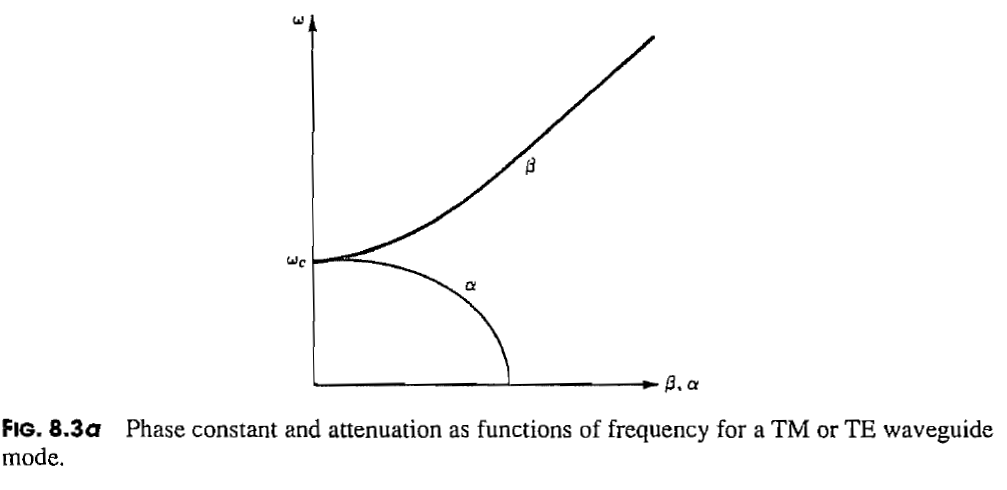
\includegraphics[scale = 0.7]{Phase constant and attenuation in parallel waveguide.PNG}
\end{figure}  

\footnote{FWE - pag 401}

\begin{tcolorbox}
    Scritto in un'altra maniera, l'onda deve essere larga almeno $\frac{\lambda}{2}$, 
    sennò non c'è propagazione. \\
    Per approfondire: \\ 
    \url{https://www.ariparma.it/risorse/articoli/Guida%20di%20onda.pdf} 
        
\end{tcolorbox}

\begin{figure}[h]
    \centering
    \includegraphics{Frequenze di cut-off in base alla modalità della guida d'onda.PNG}
\end{figure}  


La figura indica le frequenze di cut-off di diversi modi di guida d'onda. \\ 
Tipicamente, nella $TE_{10}$: 

{
    \Large
    \begin{equation}
        \frac{b}{a} = \frac{1}{2}
    \end{equation}
}

che è il valore tipicamente utilizzato nella realtà. \\ 
Normalmente, questo tipo d'onda è progettata in modo tala che la frequenza di cut-off sia il 30 per cento sotto la frequenza operativa. \\ 
In questo modo, solo un tipo d'onda si può propagare nella guida d'onda. \\ 

\begin{figure}[h]
    \centering
    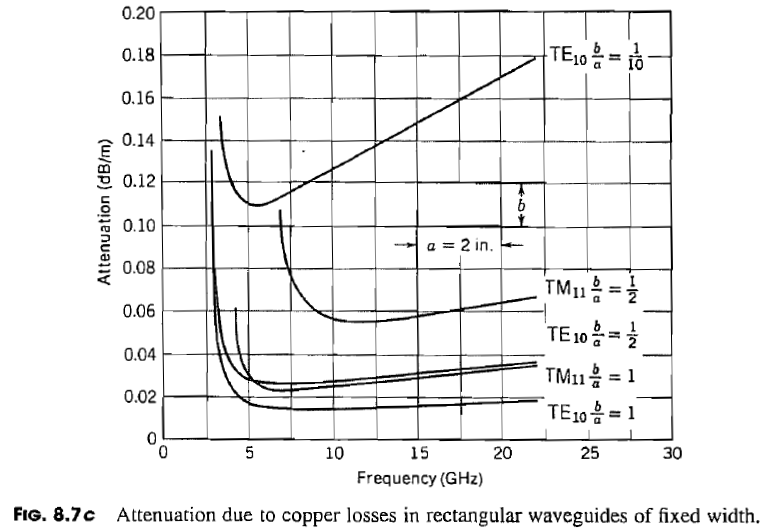
\includegraphics[scale = 0.8]{Atenuanzioni di guida d'onda con rame.PNG}
\end{figure}  



Non essendo troppo vicino alla frequenza di taglio, 
le dispersioni causate da diverse velocità di gruppo per diversi componenti di frequenze vengono minimizzati.  \\ 

Inoltre, nel modo fondamentale, la polarizzazione dei campi è fissa, 
il campo elettrico passa dal basso all'alto della guida. \\
Questa polarizzazione potrebbe essere necessaria per qualche applicazione. \\

Generalmente, viene impegato il rame come componente per le guide d'onde, e data una frequenza, l'attenuazione non è eccessivamente bassa 
rispetto a guide di altre dimensioni. \\

Nel modo fondamentale, il campo EM è il seguente: 

{
    \Large
    \begin{equation}
        \begin{cases}
            E_x = H_y = E_z = 0 \\ \\
            H_x ^{\pm} = \frac{\jmath}{\kappa_c ^{2}} \frac{\pi}{a} \beta A_{10} \sin(\frac{\pi}{a}) x e^{-\mp \jmath \beta z} \\ \\
            E_y ^{\pm} = - \frac{\jmath}{\kappa_c ^{2}} \omega \mu \frac{\pi}{a} A_{10} \sin(\frac{\pi}{a}) x e^{-\mp \jmath \beta z} 
        \end{cases}
    \end{equation}
}

in cui: 

{
    \Large 
    \begin{equation}
        \beta = \sqrt{\kappa ^{2} - (\frac{\pi}{a})^{2}}
    \end{equation}
} 

L'impedenza d'onda è uguale a: 

{
    \Large 
    \begin{equation}
        \begin{split}
            Z_{TE_{10}} 
            &= 
            - \frac{E_y}{H_x} 
            \\ 
            &= 
            \frac{\omega \mu_o}{\beta}
            \\ 
            &= 
            \frac{\omega \mu_o}{\sqrt{\kappa ^{2} - (\frac{\pi}{a})^{2}}}
        \end{split}
    \end{equation}
} 

Dal Teorema di Poynting, il flusso di potenza attiva media è:
{
    \Large
    \begin{equation}
        \begin{split}
            P_{10} 
            &= \frac{1}{2} \Re [\int_{0}^{a} \int_{0}^{b} \vec{E} \times \vec{H} ^{*} \hat{z} dx dy]
            \\ 
            &= \frac{1}{2} \Re [\int_{0}^{a} \int_{0}^{b} E_y H_x ^{*} \cdot \hat{z} dx dy]
            \\ 
            &= \frac{\omega \mu a^{3} b}{4 \pi ^{2}} \left|A_{10}\right| ^{2} \Re(\beta) 
            \\ 
            &= 
            \frac{\beta}{\omega \mu_o} \frac{\left|V^{+}\right|^{2}}{2}
        \end{split}
    \end{equation}
}


L'unico componente del campo elettrico è quello verticale $E_y$ che passa dall'alto al basso della guida. \\

$E_y$ è è massima al centro della guida e zero alle pareti della guida d'onda. \\
$H_x = 0$ alle due pareti e massimo al centro della guida, proprio come $E_y$. \\ 
$H_z$ è massima alle pareti e zero al centro. 

\begin{figure}[h]
    \centering
    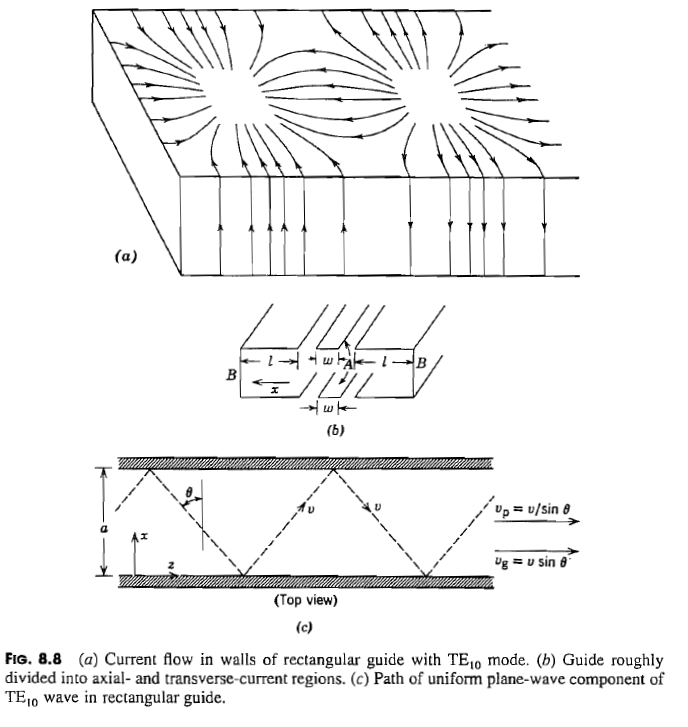
\includegraphics[scale= 0.9]{TE 10.PNG}
\end{figure}  

\newpage 

\section{Modo $TE_{20}$} 

\footnote{Slide del prof | PPT: Lezione 21 - 22 Guide rettangolari 22-24 maggio 2023 | Pag 40-42} 

Le guide d'onda sono dimensionate in modo tale che, alla frequenza di lavoro, 
ci sia solo un solo modo di propagazione, quindi: 

{
    \Large
    \begin{equation}
        a \ge 2b
    \end{equation}
}

La frequenza di cut-off per la $TE_{20}$ è: 

{
    \Large 
    \begin{equation}
        f_{c_{20}} [GHz] = \frac{300}{a [mm]}
    \end{equation}
}

Quindi l'intervallo di monomodalità, cioè l'intervallo di frequenze in cui l'onda si può propagare 
nel sistema guida d'onda così progettato è di: 

{
    \Large 
    \begin{equation}
        \frac{300}{a [mm]} \ge f[GHz] \ge \frac{150}{a [mm]}
    \end{equation}
} 

Se $m=0$, la guida d'onda non dipende da b. \\ 

$\omega_{c_{n0}}$ aumenta al diminuire di b. \\ 

Quindi b può essere il più piccolopossibile. \\ 

Ma il campo max è inversamente proporzionale a $\sqrt{b}$ 

{
    \Large 
    \begin{equation}
        \alpha_c \approx 
        \frac{R_s}{a^{3} b \kappa \eta} (2b\pi^{2} + a^{3} \kappa^{2})
    \end{equation}
}

dove: 

{
    \Large 
    \begin{equation}
        R_s = \frac{1}{\sigma \delta}
    \end{equation}
}


Quindi tipicamente: 

{
    \Large
    \begin{equation}
        a \approx 2b
    \end{equation}
}

\newpage 

\end{document}